%
%Не забыть:
%--------------------------------------
%Вставить колонтитулы, поменять название на титульнике



%--------------------------------------

\documentclass[a4paper, 12pt]{article} 

%--------------------------------------
%Russian-specific packages
%--------------------------------------
%\usepackage[warn]{mathtext}
\usepackage[T2A]{fontenc}
\usepackage[utf8]{inputenc}
\usepackage[english,russian]{babel}
\usepackage[intlimits]{amsmath}
\usepackage{esint}
%--------------------------------------
%Hyphenation rules
%--------------------------------------
\usepackage{hyphenat}
\hyphenation{ма-те-ма-ти-ка вос-ста-нав-ли-вать}
%--------------------------------------
%Packages
%--------------------------------------
\usepackage{amsmath}
\usepackage{amssymb}
\usepackage{amsfonts}
\usepackage{amsthm}
\usepackage{latexsym}
\usepackage{mathtools}
\usepackage{etoolbox}%Булевые операторы
\usepackage{extsizes}%Выставление произвольного шрифта в \documentclass
\usepackage{geometry}%Разметка листа
\usepackage{indentfirst}
\usepackage{wrapfig}%Создание обтекаемых текстом объектов
\usepackage{fancyhdr}%Создание колонтитулов
\usepackage{setspace}%Настройка интерлиньяжа
\usepackage{lastpage}%Вывод номера последней страницы в документе, \lastpage
\usepackage{soul}%Изменение параметров начертания
\usepackage{hyperref}%Две строчки с настройкой гиперссылок внутри получаеммого
\usepackage[usenames,dvipsnames,svgnames,table,rgb]{xcolor}% pdf-документа
\usepackage{multicol}%Позволяет писать текст в несколько колонок
\usepackage{cite}%Работа с библиографией
\usepackage{subfigure}% Человеческая вставка нескольких картинок
\usepackage{tikz}%Рисование рисунков
\usepackage{float}
% Для картинок Моти
\usepackage{misccorr}
\usepackage{lscape}
\usepackage{cmap}


\usepackage{graphicx,xcolor}
\graphicspath{{Pictures/}}
\DeclareGraphicsExtensions{.pdf,.png,.jpg}

%----------------------------------------
%Список окружений
%----------------------------------------
\newenvironment {theor}[2]
{\smallskip \par \textbf{#1.} \textit{#2}  \par $\blacktriangleleft$}
{\flushright{$\blacktriangleright$} \medskip \par} %лемма/теорема с доказательством
\newenvironment {proofn}
{\par $\blacktriangleleft$}
{$\blacktriangleright$ \par} %доказательство
%----------------------------------------
%Список команд
%----------------------------------------
\newcommand{\grad}
{\mathop{\mathrm{grad}}\nolimits} %градиент

\newcommand{\diver}
{\mathop{\mathrm{div}}\nolimits} %дивергенция

\newcommand{\Def}[1]
{\underline{\textbf{#1}}} %определение

\newcommand{\RN}[1]
{\MakeUppercase{\romannumeral #1}} %римские цифры

\newcommand {\theornp}[2]
{\textbf{#1.} \textit{ #2} \par} %Написание леммы/теоремы без доказательства

\newcommand{\qrq}
{\ensuremath{\quad \Rightarrow \quad}} %Человеческий знак следствия

\newcommand{\qlrq}
{\ensuremath{\quad \Leftrightarrow \quad}} %Человеческий знак равносильности

\renewcommand{\phi}{\varphi} %Нормальный знак фи

\newcommand{\me}
{\ensuremath{\mathbb{E}}}

\newcommand{\md}
{\ensuremath{\mathbb{D}}}



%\renewcommand{\vec}{\overline}




%----------------------------------------
%Разметка листа
%----------------------------------------
\geometry{top = 3cm}
\geometry{bottom = 2cm}
\geometry{left = 1.5cm}
\geometry{right = 1.5cm}
%----------------------------------------
%Колонтитулы
%----------------------------------------
\pagestyle{fancy}%Создание колонтитулов
\fancyhead{}
%\fancyfoot{}
\fancyhead[R]{\textsc{Гистерезис}}%Вставить колонтитул сюда
%----------------------------------------
%Интерлиньяж (расстояния между строчками)
%----------------------------------------
%\onehalfspacing -- интерлиньяж 1.5
%\doublespacing -- интерлиньяж 2
%----------------------------------------
%Настройка гиперссылок
%----------------------------------------
\hypersetup{				% Гиперссылки
	unicode=true,           % русские буквы в раздела PDF
	pdftitle={Заголовок},   % Заголовок
	pdfauthor={Автор},      % Автор
	pdfsubject={Тема},      % Тема
	pdfcreator={Создатель}, % Создатель
	pdfproducer={Производитель}, % Производитель
	pdfkeywords={keyword1} {key2} {key3}, % Ключевые слова
	colorlinks=true,       	% false: ссылки в рамках; true: цветные ссылки
	linkcolor=blue,          % внутренние ссылки
	citecolor=blue,        % на библиографию
	filecolor=magenta,      % на файлы
	urlcolor=cyan           % на URL
}
%----------------------------------------
%Работа с библиографией (как бич)
%----------------------------------------
\renewcommand{\refname}{Список литературы}%Изменение названия списка литературы для article
%\renewcommand{\bibname}{Список литературы}%Изменение названия списка литературы для book и report
%----------------------------------------
\begin{document}
	\begin{titlepage}
		\begin{center}
			$$$$
			$$$$
			$$$$
			$$$$
			{\Large{НАЦИОНАЛЬНЫЙ ИССЛЕДОВАТЕЛЬСКИЙ УНИВЕРСИТЕТ}}\\
			\vspace{0.1cm}
			{\Large{ВЫСШАЯ ШКОЛА ЭКОНОМИКИ}}\\
			\vspace{0.25cm}
			{\large{Факультет физики}}\\
			\vspace{5.5cm}
			{\Huge\textbf{{Лабораторная работа}}}\\%Общее название
			\vspace{1cm}
			{\LARGE{<<Гистерезис>>}}\\%Точное название
			\vspace{2cm}
			{Работу выполнил студент 2 курса}\\
			{Захаров Сергей Дмитриевич}
			\vfill
			
\includegraphics[width = 0.2\textwidth]{HSElogo}\\
			\vfill
			Москва\\
			2019
		\end{center}
	\end{titlepage}


\tableofcontents

\newpage

\section{Цель работы}

Перед началом выполнения работы были поставлены следующие цели:

\begin{enumerate}
	\item Изготовить катушку индуктивности с ферритовым сердечником и измерить ее индуктивность и магнитную восприимчивость.
	
	\item Пронаблюдать петлю магнитного гистерезиса и измерить на ее основании магнитные параметры материала сердечника.
\end{enumerate}

\section{Описание метода выполнения работы}

\subsection{Получение характеристик катушки}

Сперва было решено определиться с тем, каким образом будет найдена индуктивность. С этой целью была собрана схема, представленная на рисунке \ref{fig:circuit_L}.

\begin{figure}[H]
	\centering
	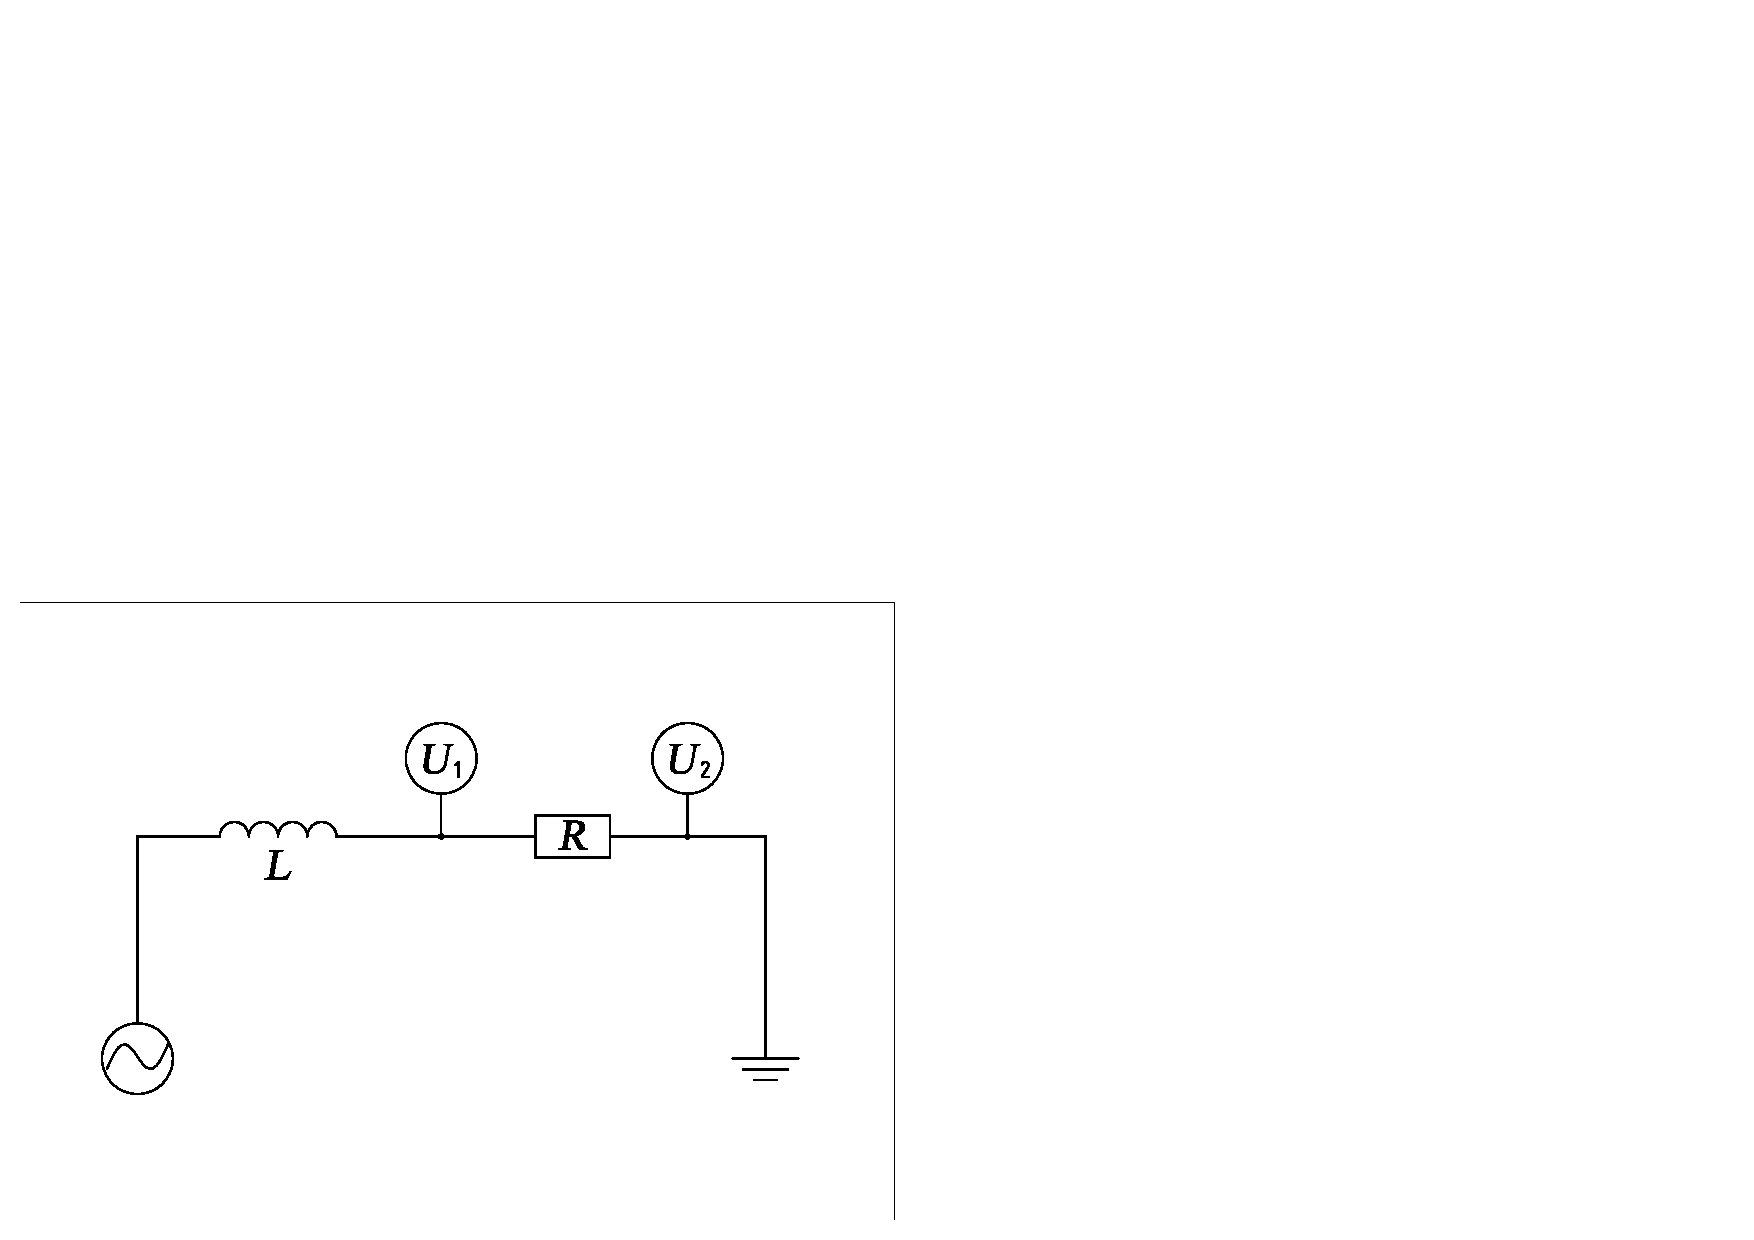
\includegraphics[width=0.7\textwidth]{Hysteresis_circuit_2}
	\caption{Схема для определения индуктивности катушки}
	\label{fig:circuit_L}
\end{figure}

Для того, чтобы с ее помощью измерить индуктивность, обратимся к следующим выкладкам:

\begin{equation*}
	\frac{U_1}{U_2} = \sqrt{1 + \left(\frac{\omega L}{R}\right)^2}
\end{equation*}

На основании этого получаем формулу для расчета индуктивности:

\begin{equation}
	\label{eq:L}
	L = \frac{R}{\omega} \cdot \sqrt{\left(\frac{U_1}{U_2}\right)^2 - 1}
\end{equation}

Помимо нахождения индуктивности, в лабораторной также предполагалось нахождение магнитной восприимчивости сердечника. Для того, чтобы это сделать, обратимся к следующей формуле:

\begin{equation*}
	L = \mu_0 \cdot \mu \cdot h \cdot \frac{N^2}{2\cdot \pi} \cdot \ln\frac{D}{d}
\end{equation*}

Здесь $N$ --- число витков катушки, $h$ --- ее высота, $\mu_0$ --- магнитная постоянная, $D$ --- внешний диаметр, $d$ --- внутренний диаметр.

Таким образом, получаем:

\begin{equation}
	\label{eq:chi}
	\mu = \frac{L \cdot 2 \cdot \pi}{\mu_0 \cdot h \cdot N^2 \cdot \ln \dfrac{D}{d}}
\end{equation}

\subsection{Наблюдение петли магнитного гистерезиса}

Для наблюдения петли гистерезиса была предложена схема, представленная на рисунке \ref{fig:circuit_loop}.

\begin{figure}[H]
	\centering
	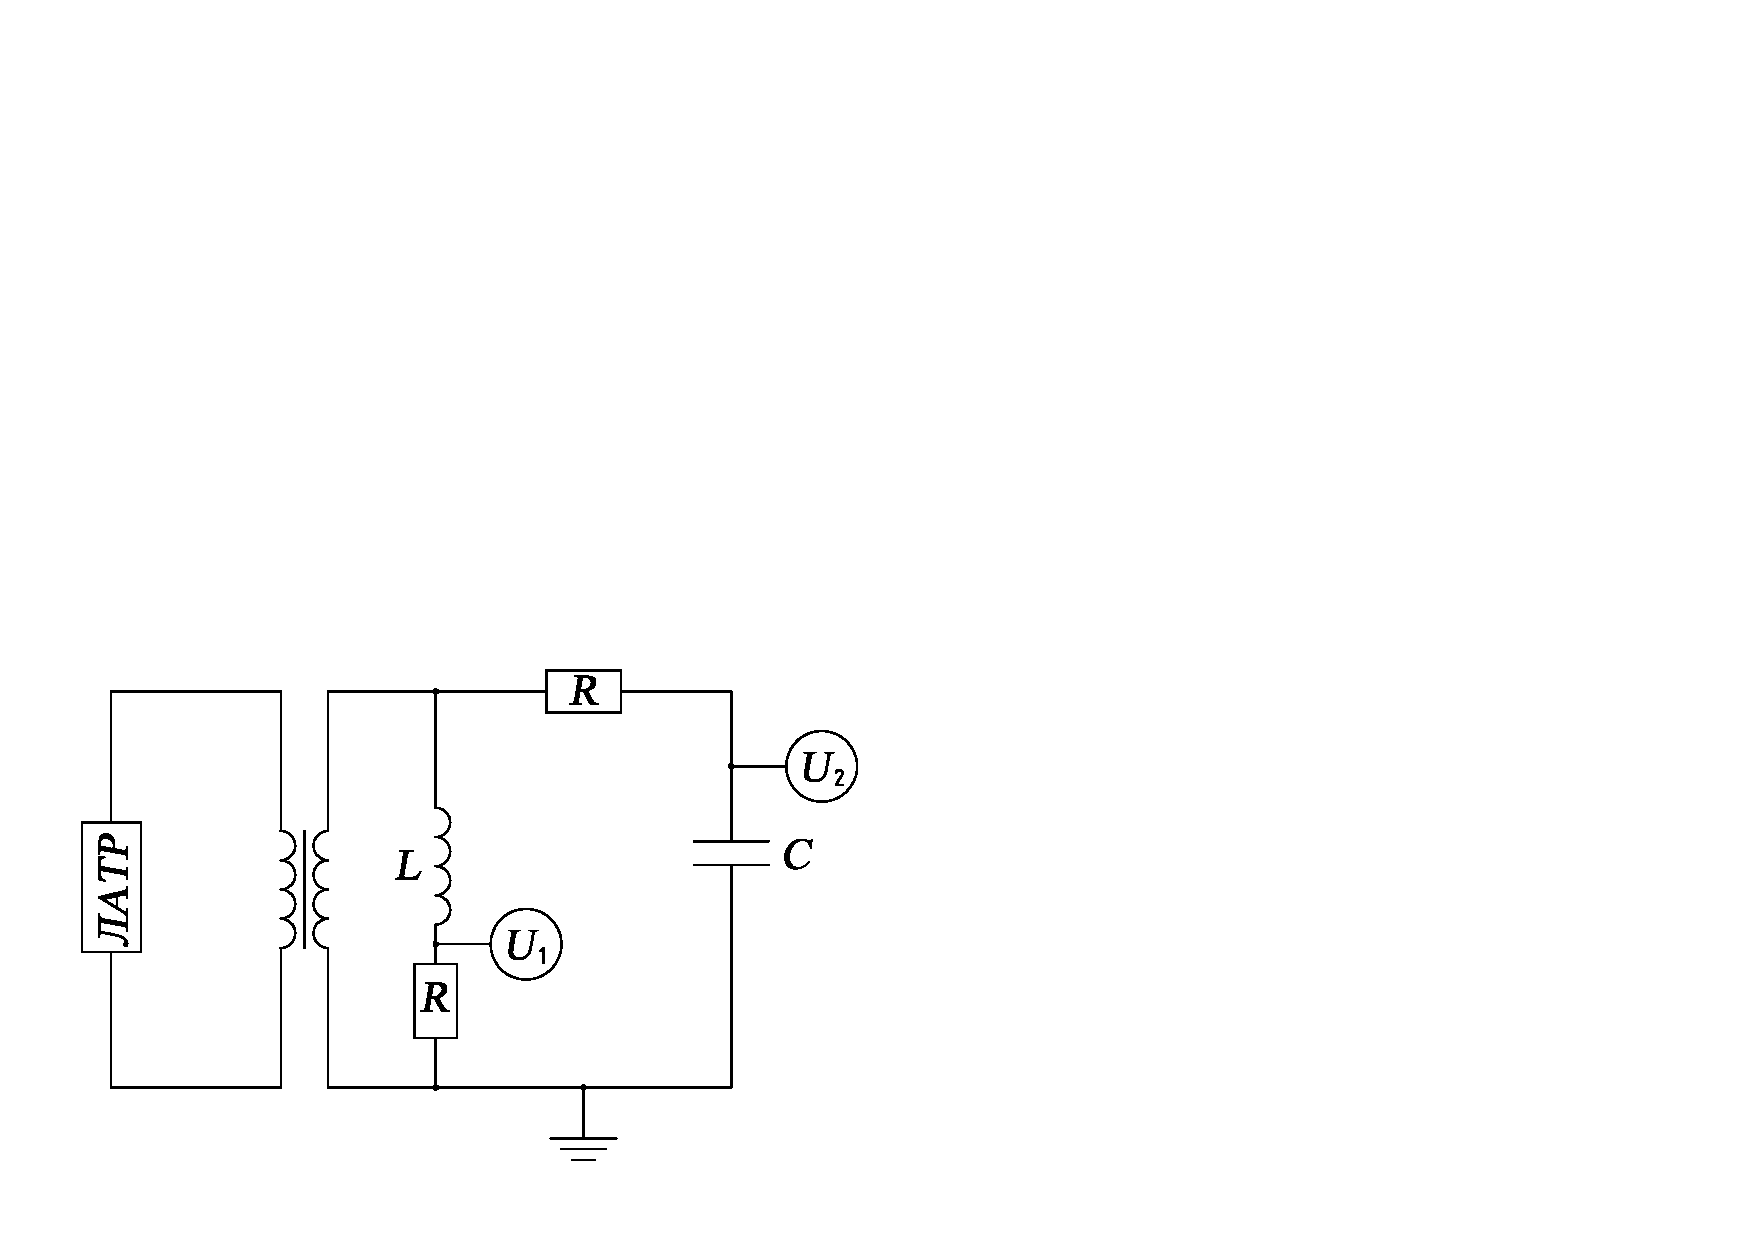
\includegraphics[width=0.7\textwidth]{Hysteresis_circuit_1}
	\caption{Схема для наблюдения петли гистерезиса}
	\label{fig:circuit_loop}
\end{figure}

Резистор с малым сопротивлением необходим для измерения тока в цепи с помощью напряжения $U_1$. 

При знании тока, текущего через катушку, можно выразить напряженность поля в ней с помощью теоремы о циркуляции:

\begin{equation}
	\label{eq:H}
	H = \frac{N \cdot I}{\pi\cdot D} = \frac{N \cdot U_1}{\pi\cdot D\cdot R}
\end{equation}

Здесь $N$ --- число витков катушки, $D$ --- средний диаметр сердечника, $R$ --- сопротивление резистора с малым сопротивлением.

Для того, чтобы выразить индукция поля, можно воспользоваться законом Фарадея:

\begin{equation}
	\label{eq:faradey}
	U = -\frac{d\Phi}{dt} = - S \cdot N \cdot \frac{dB}{dt}
\end{equation}

В целом нетрудно показать, что в нашем случае также верно, что напряжение на конденсаторе можно записать следующим образом:

\begin{equation}
	\label{eq:Ucap}
	U_2 = \frac{1}{R_b\cdot C} \cdot \int U dt = \frac{1}{R_b \cdot C}\cdot S \cdot N \cdot B
\end{equation}

На основании этой связи получаем следующее выражение для индукции:

\begin{equation}
	\label{eq:B}
	B = \frac{R_b \cdot C \cdot U_2}{S \cdot N}
\end{equation}

Здесь $R_b$ --- величина большого сопротивления, подключенного к конденсатору, $C$ --- емкость конденсатора, $S$ --- площадь поперечного сечения сердечника катушки, $N$ --- число витков катушки. 

Наконец, было решено получить значение остаточной намагниченности катушки --- намагниченности, которую имеет ферромагнитный материал при напряженности поля, равной нулю. Строго говоря, намагниченность не является тем же самым, что и индукция, однако отличаются эти величины лишь постоянным коэффициентом, поэтому отождествим эти величины и обозначим остаточную намагниченность как $B_r$.

Аналогичным образом можно определить и коэрцитивную силу (значение напряжённости магнитного поля, необходимое для полного размагничивания объекта) как напряженность поля $H_r$ при индукции, равной нулю.


\section{Выполнение работы}

\subsection{Определение характеристик катушки}

Сперва нами было создано две катушки с сердечниками различных размеров (однако, оба из них были ферритовые). Данные об этих катушках приведены ниже.


\begin{center}
\begin{tabular}{|c|c|c|}
	\hline 
	Параметр & Первая катушка & Вторая катушка \\ 
	\hline 
	Число витков & 30  & 36 \\ 
	\hline 
	Высота сердечника, мм & $12 \pm 0.2$ & $7 \pm 0.2$ \\ 
	\hline 
	Толщина сердечника, мм & $8.5\pm 0.2$ & $7 \pm 0.2$\\ 
	\hline 
	Внешний диаметр сердечника, мм & $45 \pm 0.2$ & $38 \pm 0.2$ \\ 
	\hline 
	Средний диаметр сердечника, мм & $36.5 \pm 0.2$ & $31 \pm 0.2$ \\ 
	\hline 
	Длина сердечника, мм & $114.67 \pm 0.2$ & $97.39 \pm 0.2$ \\ 
	\hline 
\end{tabular} 
	
\end{center}

\medspace

На основании полученных данных с помощью формулы (\ref{eq:L}) были получены зависимости индуктивностей катушек от частоты колебаний источника, представленные на рисунках \ref{fig:inductivity1} и \ref{fig:inductivity2} соответственно.

\begin{figure}[H]
	\centering
	\subfigure[]{
	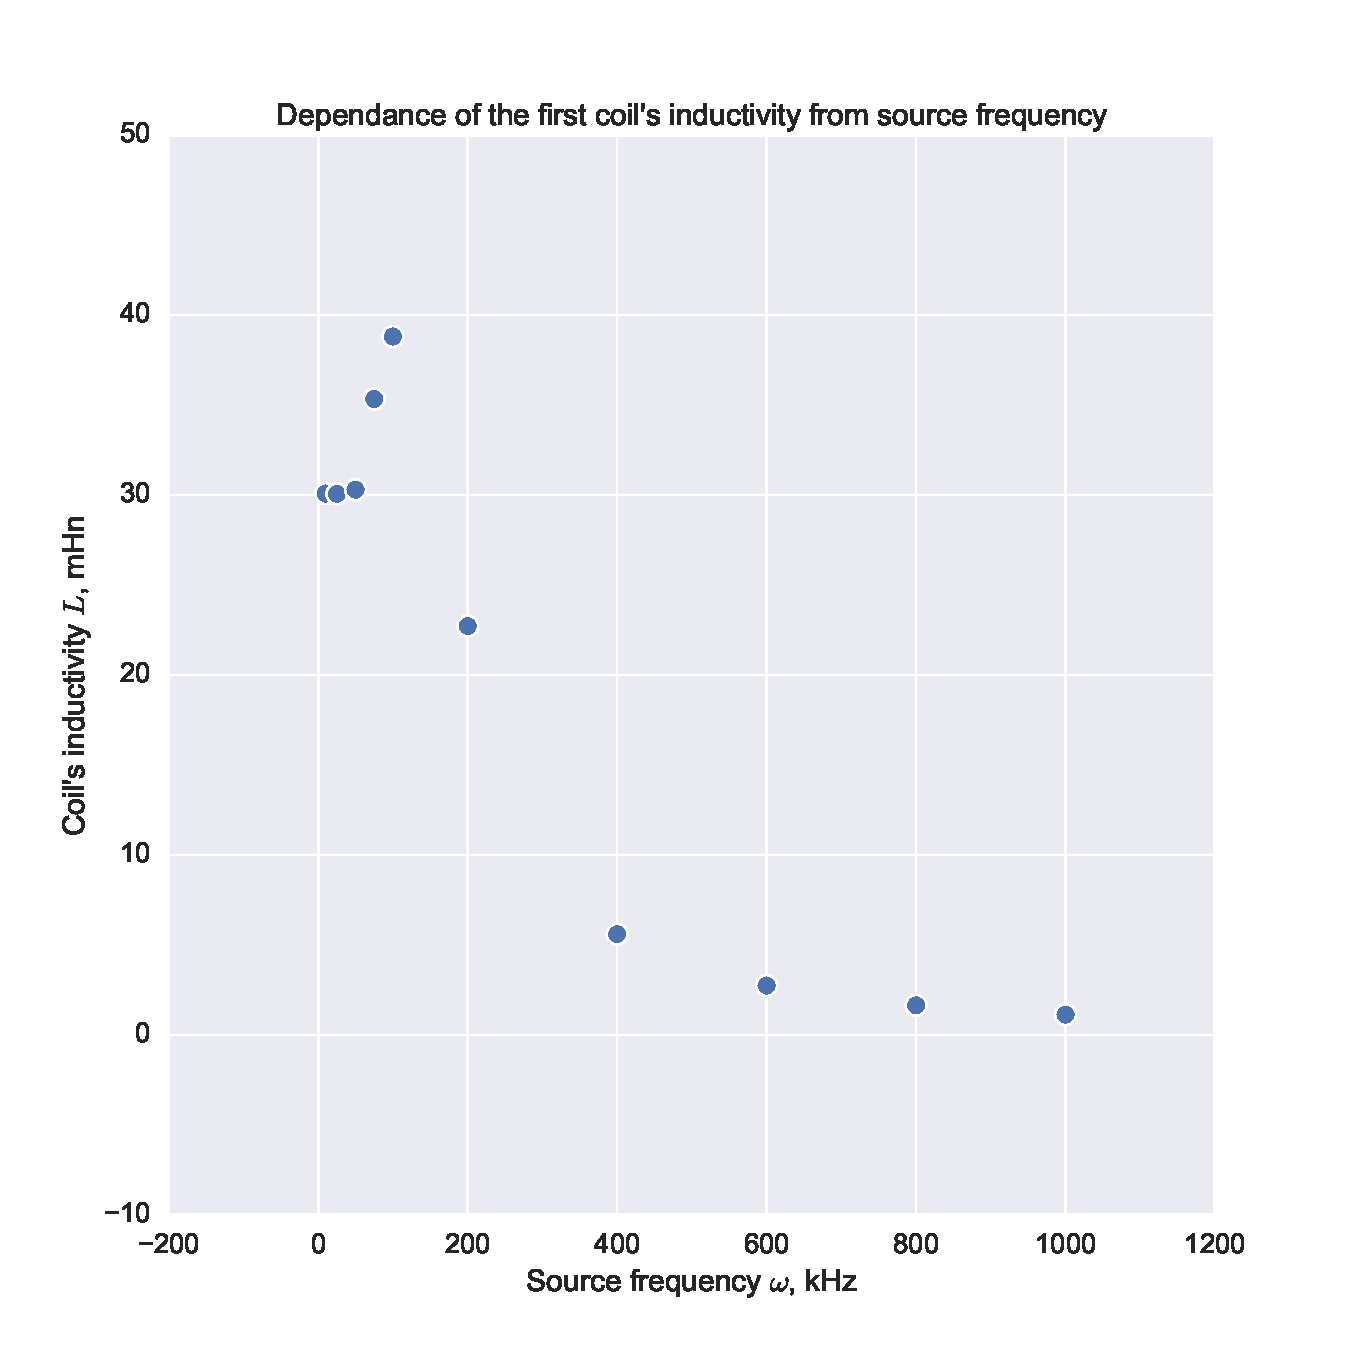
\includegraphics[width=0.48\textwidth]{Inductivity_1}
	\label{fig:inductivity1}}
	\subfigure[]{
	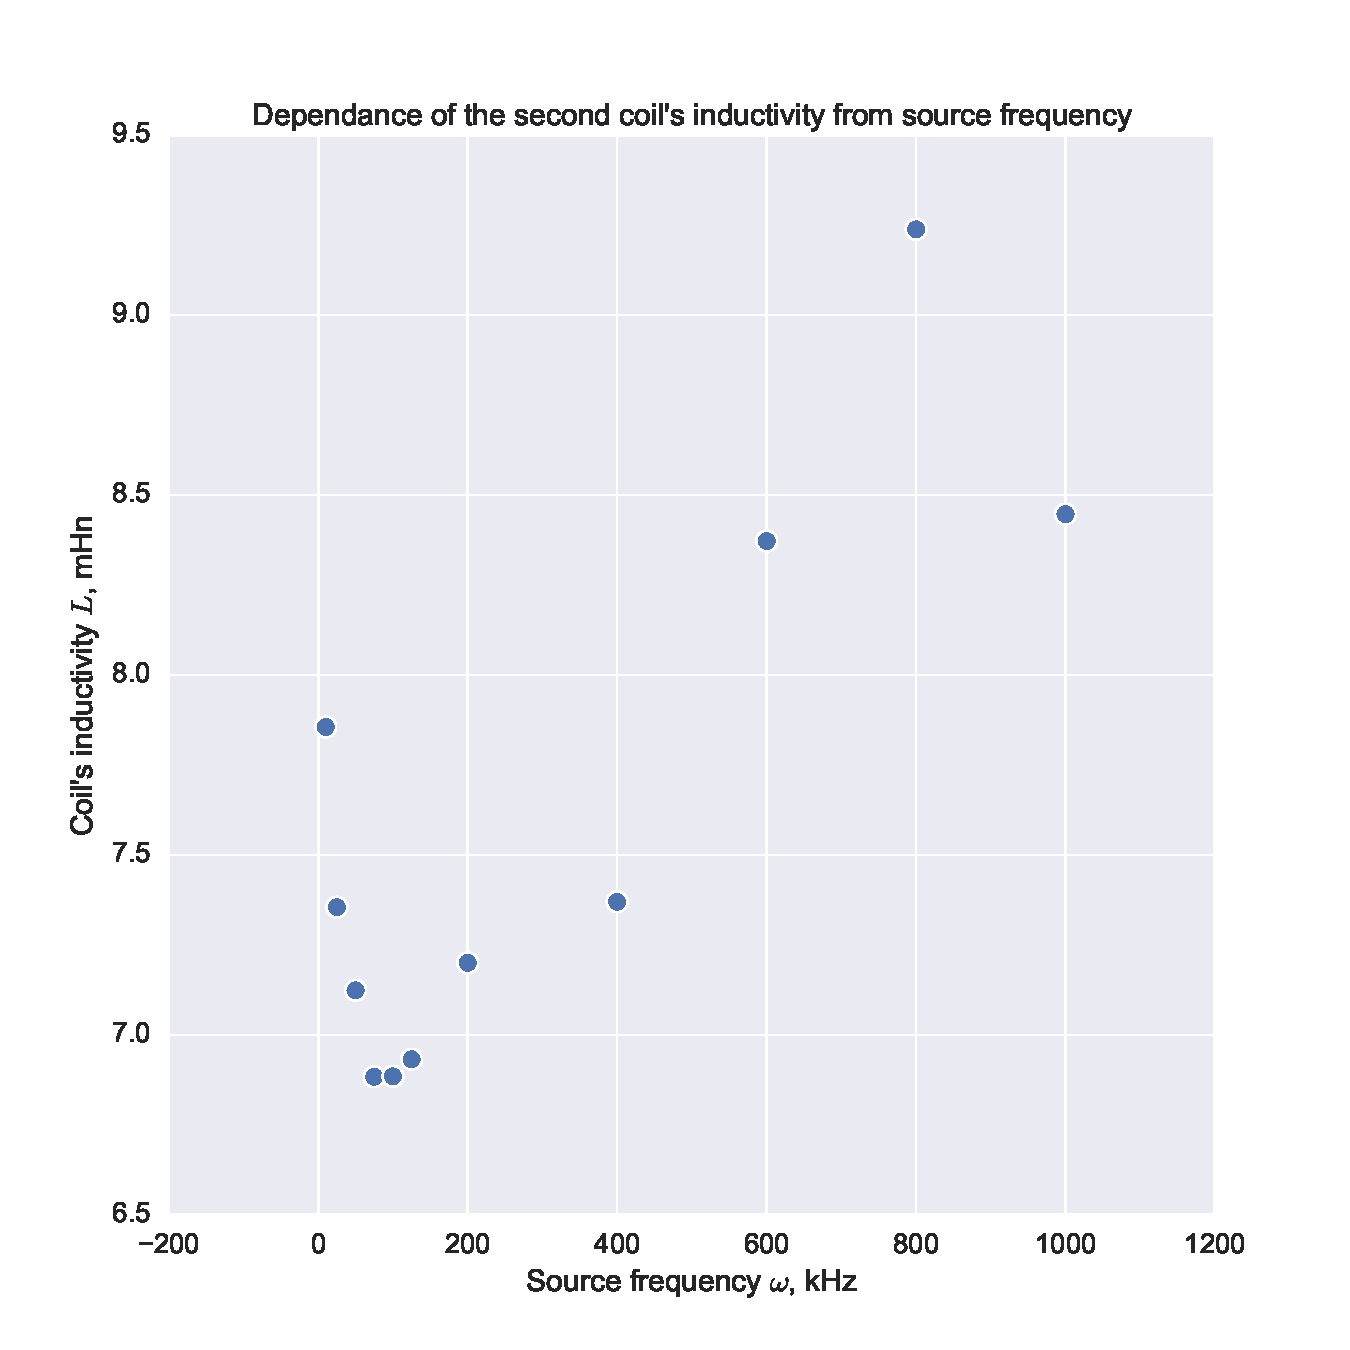
\includegraphics[width=0.48\textwidth]{Inductivity_2}
	\label{fig:inductivity2}}
	\caption{Зависимость индуктивности катушки 1 \subref{fig:inductivity1} и катушки 2 \subref{fig:inductivity2} от частоты источника}
\end{figure}

Кроме того, зная индуктивность, возможно построить и зависимость магнитной восприимчивости материала сердечника, воспользовавшись формулой \ref{eq:chi}. Полученные зависимости отображены на рисунках \ref{fig:mu1} и \ref{fig:mu2}.

\begin{figure}[H]
	\centering
	\subfigure[]{
	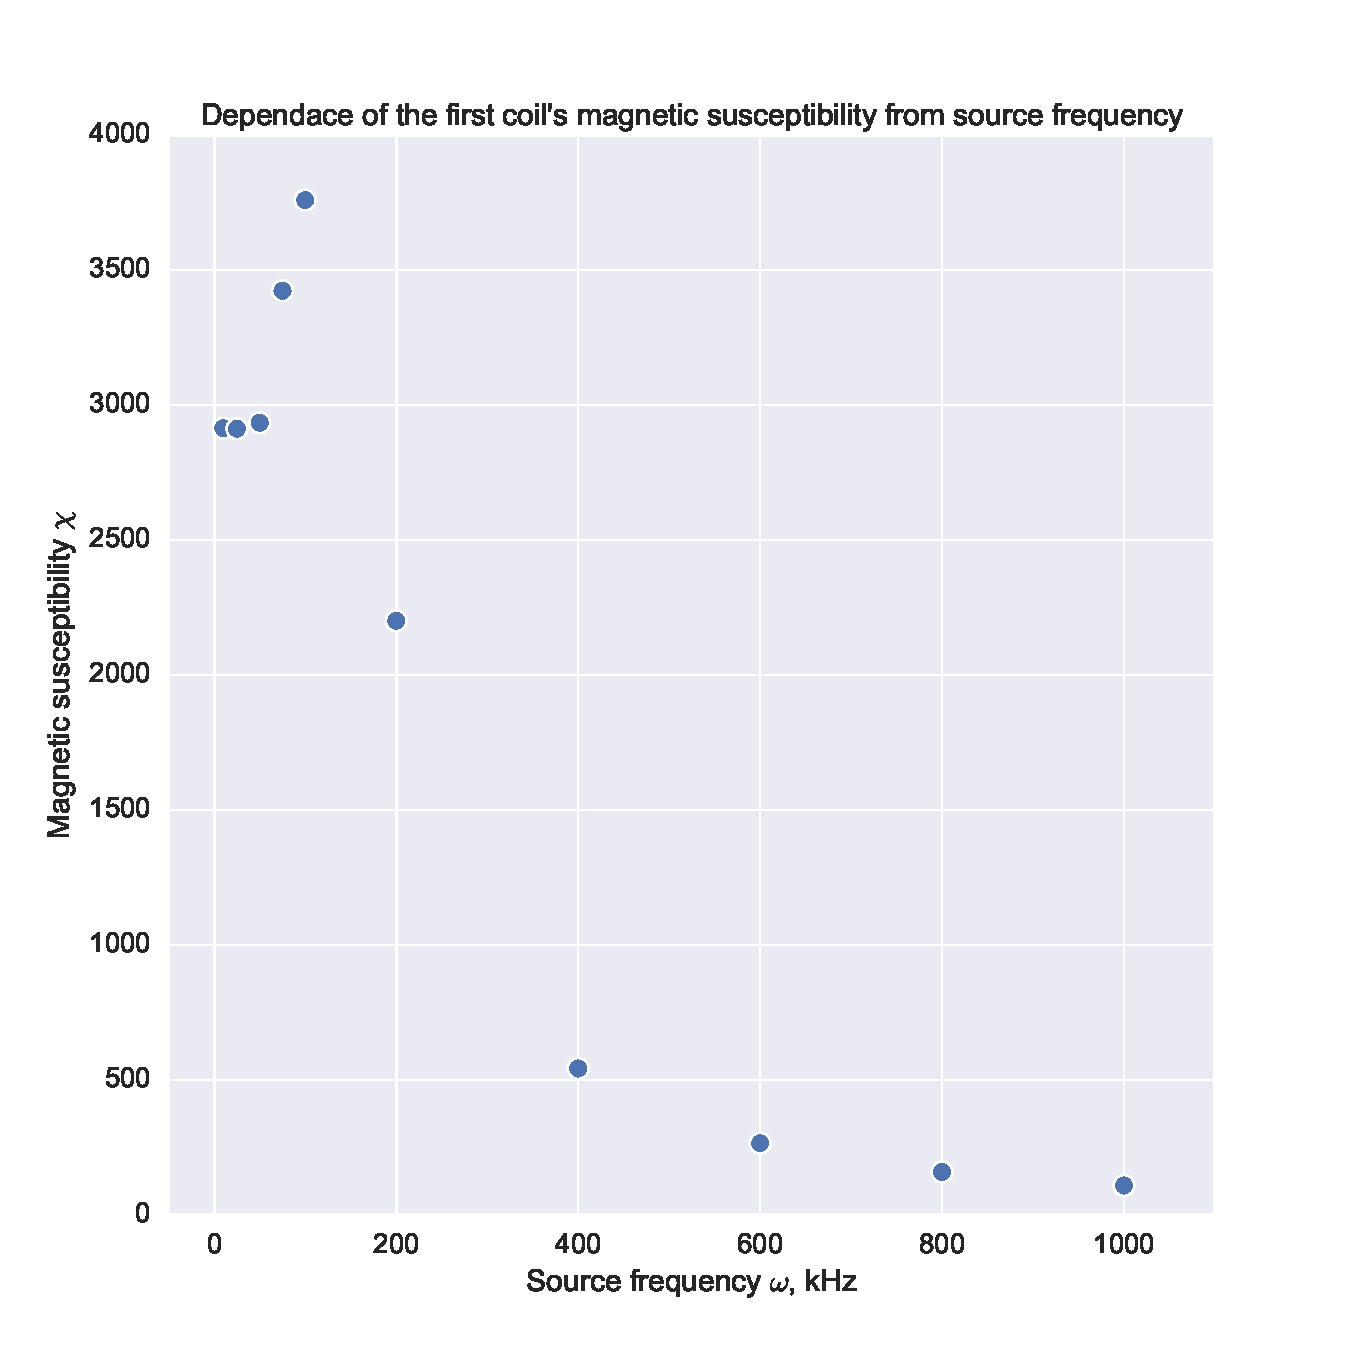
\includegraphics[width=0.48\textwidth]{Mu1}
	\label{fig:mu1}}
	\subfigure[]{
	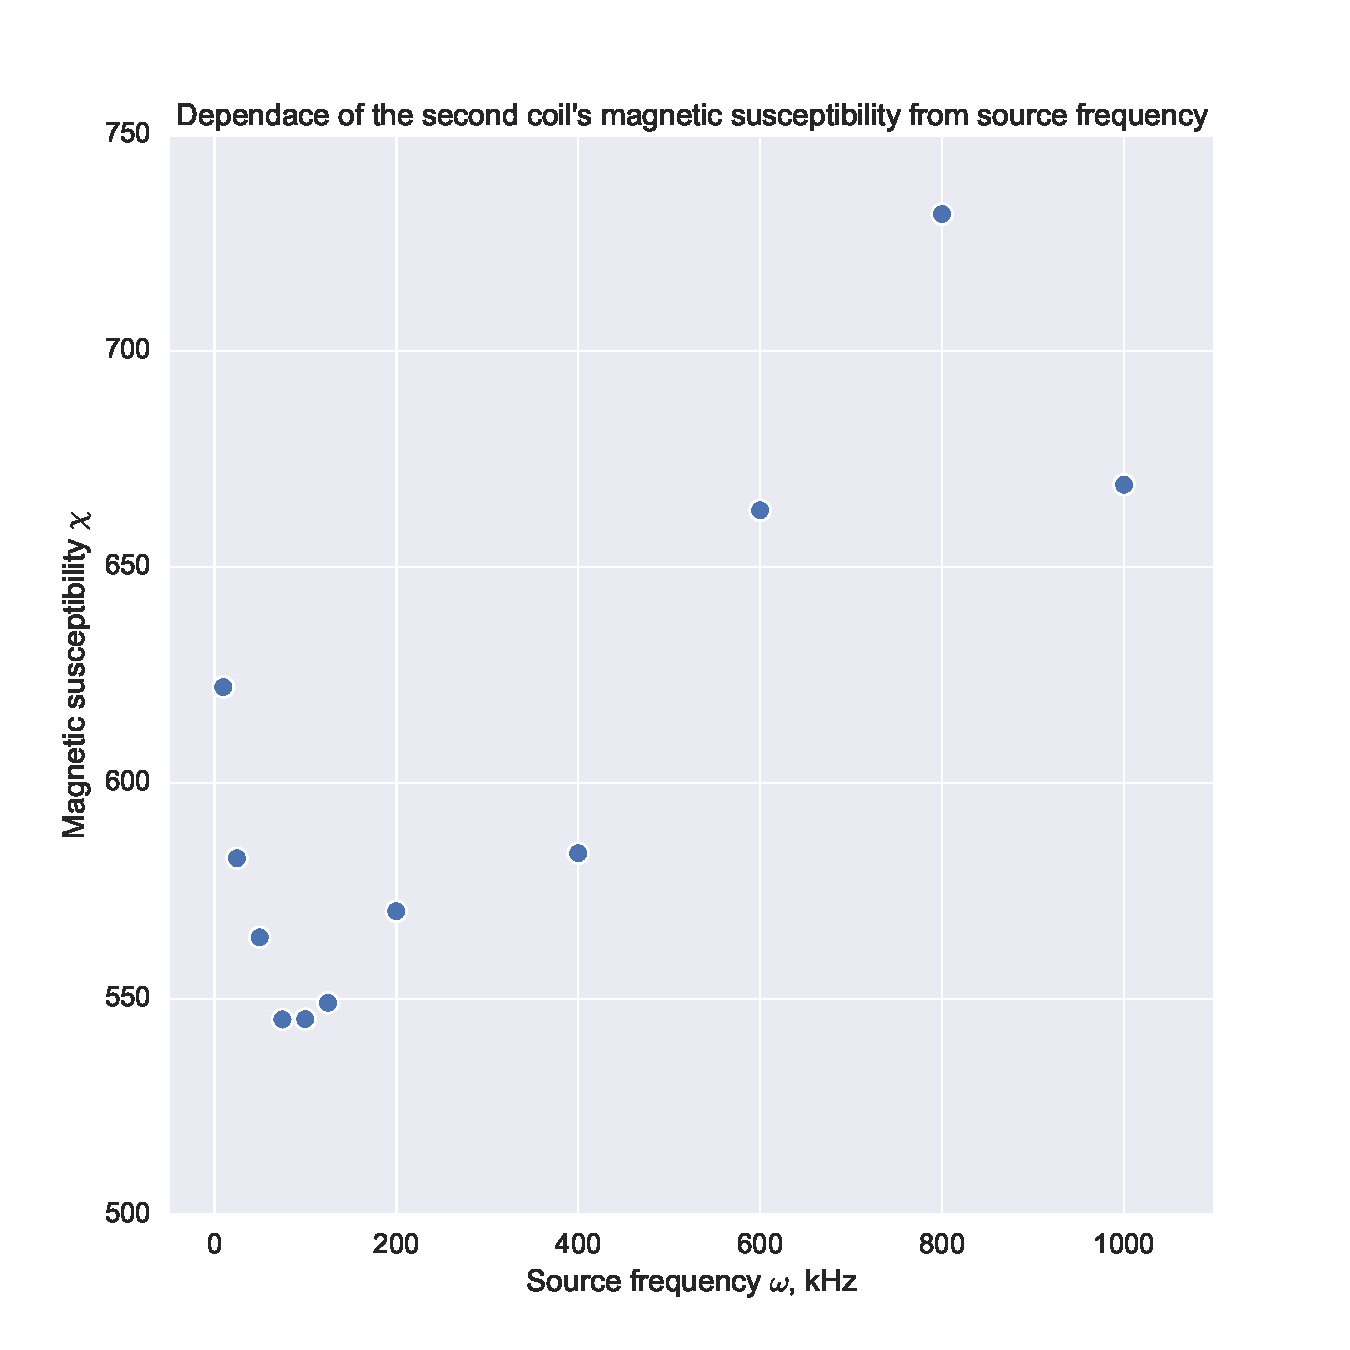
\includegraphics[width=0.48\textwidth]{Mu2}
	\label{fig:mu2}}
	\caption{Зависимость магнитной проницаемости катушек 1 \subref{fig:mu1} и 2 \subref{fig:mu2} от частоты источника}
\end{figure}

\subsection{Работа с наблюдаемой петлей магнитного гистерезиса}

С помощью схемы, представленной на рисунке \ref{fig:circuit_loop}, а также формул (\ref{eq:B}) и (\ref{eq:H}) для каждой из катушек была получена петля магнитного гистерезиса. Петли представлены на рисунках \ref{fig:Hysteresis_1} и \ref{fig:Hysteresis_2}.

\begin{figure}[H]
	\centering
	\subfigure[]{
	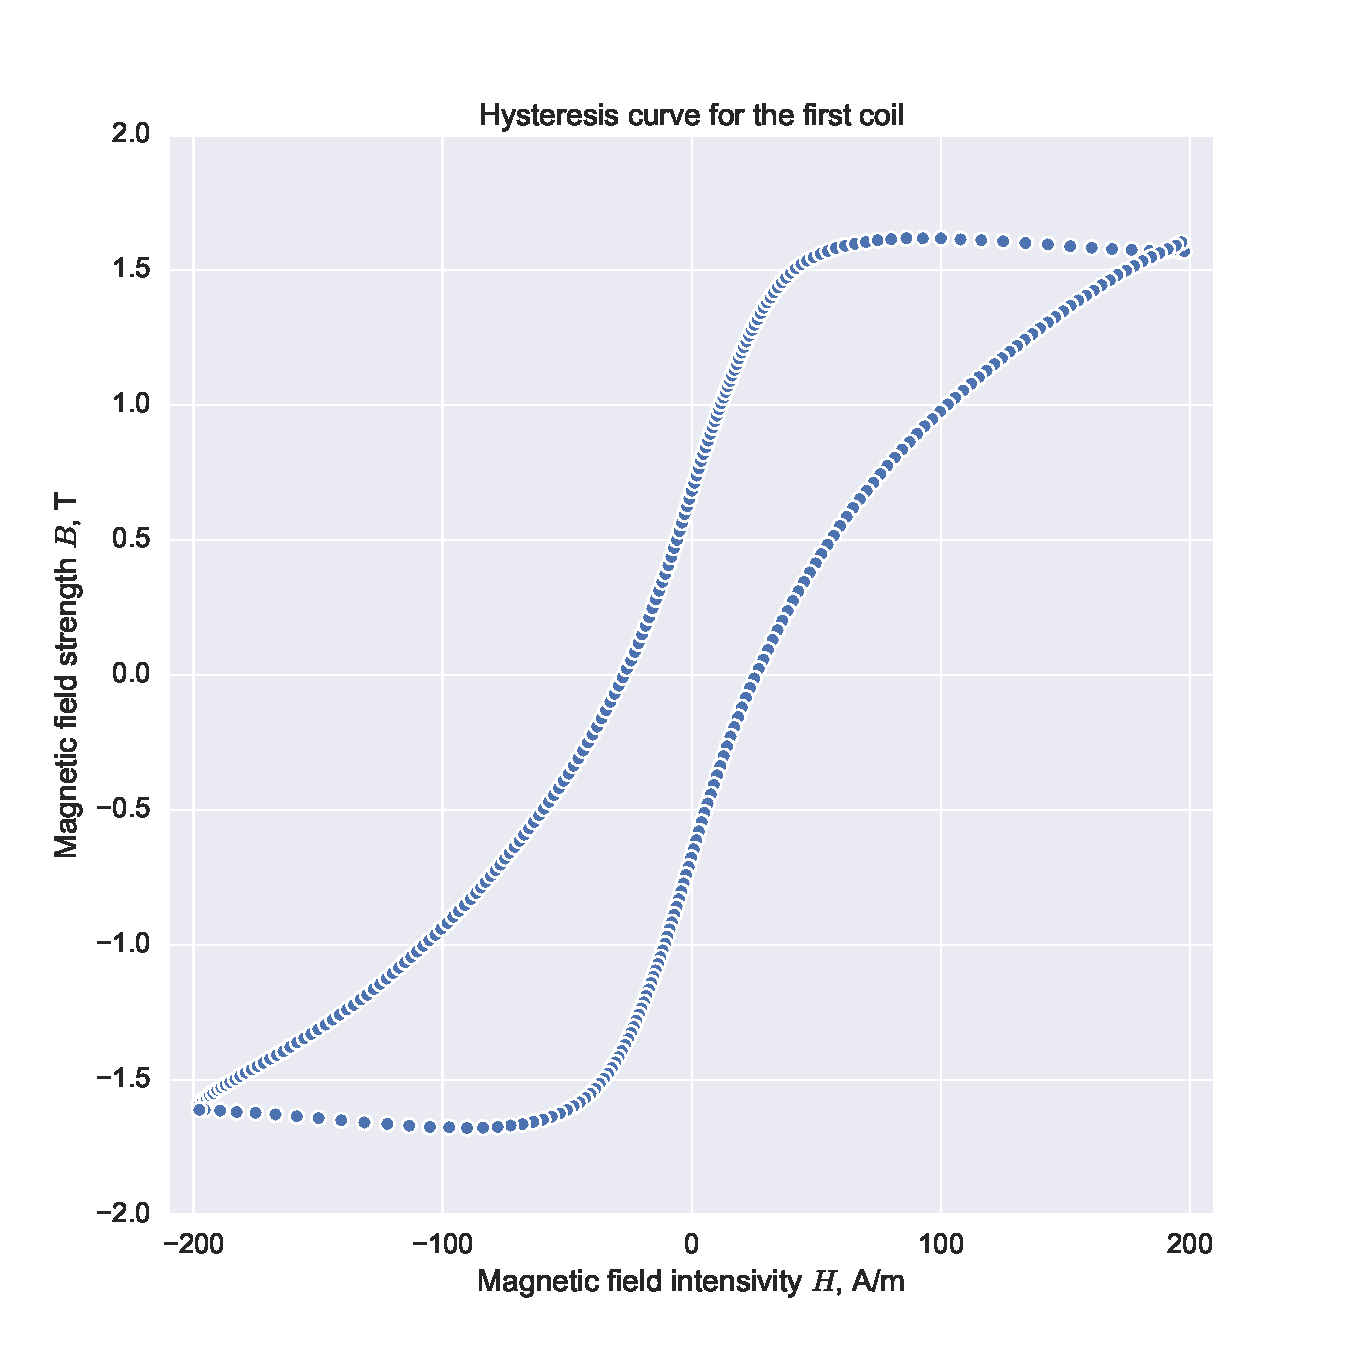
\includegraphics[width=0.48\textwidth]{Hysteresis_1}
	\label{fig:Hysteresis_1}}
	\subfigure[]{
	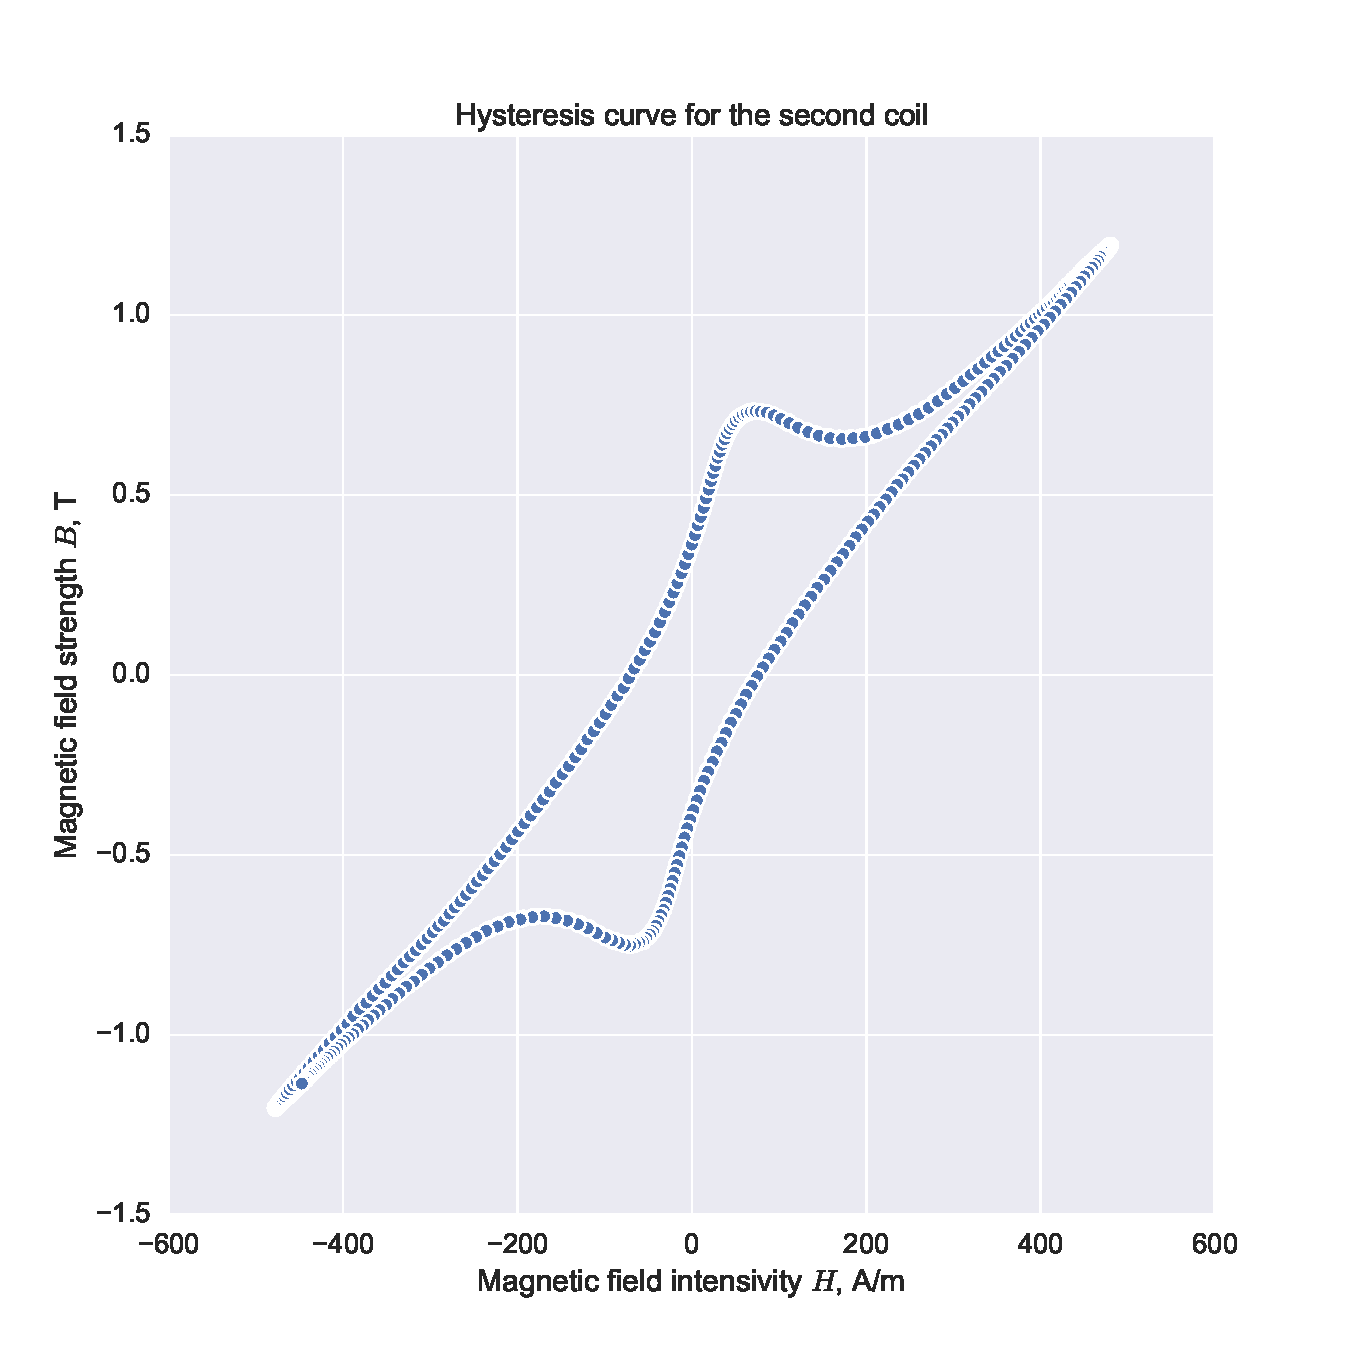
\includegraphics[width=0.48\textwidth]{Hysteresis_2}
	\label{fig:Hysteresis_2}}
	\caption{Петли магнитного гистерезиса первой \subref{fig:Hysteresis_1} и второй \subref{fig:Hysteresis_2} катушек.}
\end{figure}

На основании изложенной теории было также установлено, что для первой катушки остаточная намагниченность равна $\boxed{B_{r1} = 0.68 \pm 0.04 \text{ Тл}}$, для второй катушки $\boxed{B_{r2} = 0.35 \pm 0.031 \text{ Тл}}$. Коэрцитивные силы оказались равны $\boxed{H_{r1} = 24.4 \pm  0.53 \text{ А/м}}$ и $\boxed{H_{r2} = 87.4 \pm 0.5\text{ А/м}}$.

\section{Заключение} %Дописать

\begin{enumerate}
	\item В ходе работы было установлено, что для небольших частот индуктивность катушек равна соответственно $30$ мГн и $70$ мГн.
	
	\item  Для одной из катушек также получилось пронаблюдать т.н. кривую Столетова.
	
	\item Удалось пронаблюдать петлю гистерезиса
	
	\item Была определена остаточная намагниченность, равная $B_{r1} = 0.68 \pm 0.04$ Тл и $B_{r2} = 0.35 \pm 0.031$ Тл для первой и второй катушек соответственно.
	
	\item Была определена коэрцитивная сила, равная $H_{r1} = 24.4 \pm 0.53\text{ А/м} $ и $H_{r2} = 87.4 \pm 0.5\text{ А/м}$ для первой и второй катушек соответственно. 
\end{enumerate}















\end{document}





















